\chapter{Оптимизация сетей систем массового обслуживания}

\section{Постановка задачи}

\subsubsection{Вариант 030}

Задача №2.

\begin{figure}[h!]
	\centering
	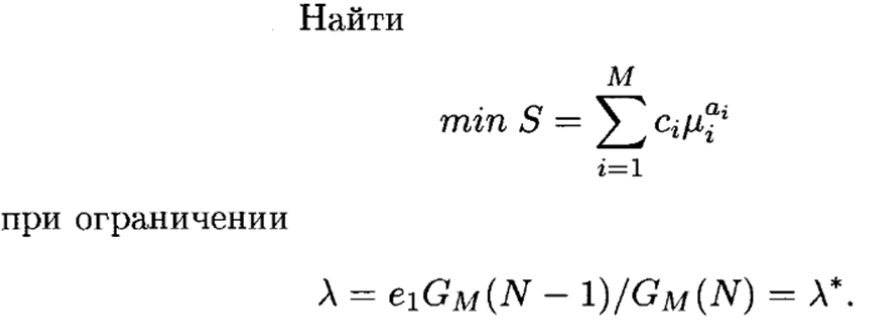
\includegraphics[scale = 0.39]{images/p3_1.png}
	\label{image:p3_1}
\end{figure}

\begin{figure}[h!]
	\centering
	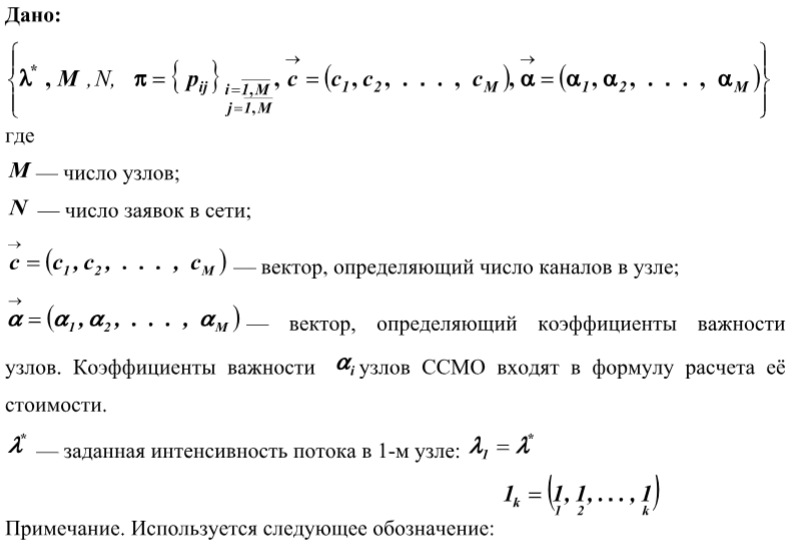
\includegraphics[scale = 0.59]{images/p3_2.png}
	\label{image:p3_2}
\end{figure}

\begin{figure}[h!]
	\centering
	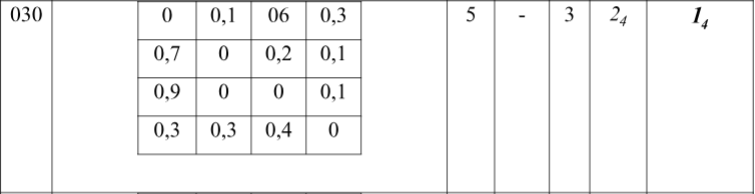
\includegraphics[scale = 0.59]{images/p3_3.png}
	\label{image:p3_3}
\end{figure}

\section{Решение}

\subsection{Методика решения простыми итерациями}

Задача оптимизации замкнутой однородной сети сводится к решению системы системы нелинейных уравнений:

\begin{figure}[h!]
	\centering
	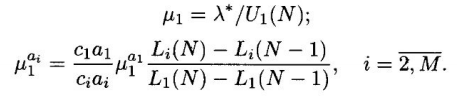
\includegraphics[scale = 0.79]{images/p3_4_r.png}
	\label{image:p3_4r}
\end{figure}

Для многоканальной сети МО используется итерационная процедура расчета среднего числа заявок в очереди. Процедура инициализируется следующими начальными условиями:

\begin{figure}[h!]
	\centering
	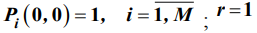
\includegraphics[scale = 0.69]{images/p3_4_0.png}
	\label{image:p3_40}
\end{figure}

Первый шаг процедуры:

\begin{figure}[h!]
	\centering
	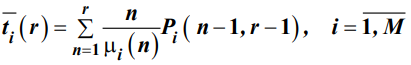
\includegraphics[scale = 0.69]{images/p3_4_1.png}
	\label{image:p3_41}
\end{figure}

\begin{figure}[h!]
	\centering
	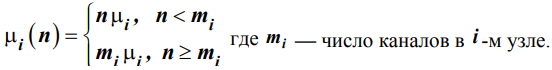
\includegraphics[scale = 0.69]{images/p3_4_m.png}
	\label{image:p3_4m}
\end{figure}

Второй шаг процедуры:

\begin{figure}[h!]
	\centering
	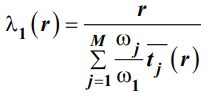
\includegraphics[scale = 0.69]{images/p3_4_2.png}
	\label{image:p3_42}
\end{figure}

Третий шаг процедуры:

\begin{figure}[h!]
	\centering
	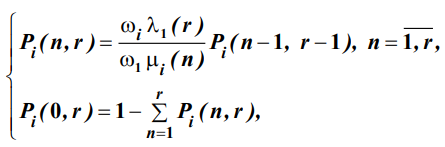
\includegraphics[scale = 0.69]{images/p3_4_3.png}
	\label{image:p3_43}
\end{figure}

\clearpage

После этого значение r увеличивается на единицу до достижения N. В результате работы процедуры формируются значения следующих характеристик:

\begin{figure}[h!]
	\centering
	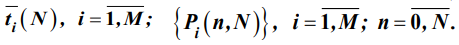
\includegraphics[scale = 0.69]{images/p3_4_4.png}
	\label{image:p3_44}
\end{figure}

\subsection{Решение задачи методом простых итераций}

Разработаем скрипт для расчета результирующего вектора $\mu$ в среде MATLAB (Приложение 10).

Результат расчета вектора $\mu$:

\lstinputlisting{listings/p3.l1.log}

Алгоритм ожидаемо не сошелся, так как метод простых итераций не рекомендуется к использованию из-за ненадежности в плане сходимости.

\subsection{Методика решения через через нормирующую константу методом Ньютона}

Задача оптимизации замкнутой однородной сети сводится к решению системы нелинейных уравнений:

\begin{figure}[h!]
	\centering
	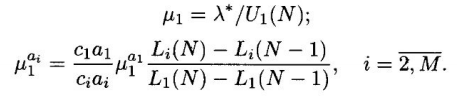
\includegraphics[scale = 0.79]{images/p3_4_r.png}
	\label{image:p3_4rx}
\end{figure}

Тогда интенсивность на выходе i -го узла однородной замкнутой сети СМО:

\begin{figure}[h!]
	\centering
	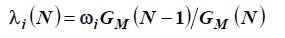
\includegraphics[scale = 0.79]{images/p3_5_1.png}
	\label{image:p3_5_1}
\end{figure}

\clearpage

Среднее число заявок в граничном узле однородной замкнутой сети СМО:

\begin{figure}[h!]
	\centering
	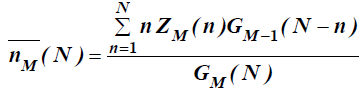
\includegraphics[scale = 0.79]{images/p3_5_2.png}
	\label{image:p3_5_2}
\end{figure}

Методика расчета нормирующей константы:

\begin{figure}[h!]
	\centering
	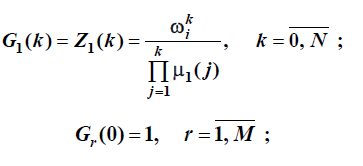
\includegraphics[scale = 0.79]{images/p3_5_4.png}
	\label{image:p3_5_4}
\end{figure}

\begin{figure}[h!]
	\centering
	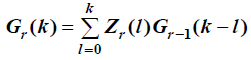
\includegraphics[scale = 0.79]{images/p3_5_5.png}
	\label{image:p3_5_5}
\end{figure}

Алгоритм Ньютона для решения системы нелинейных уравнений (W -- матрица якоби для системы уравнений F):

\begin{figure}[h!]
	\centering
	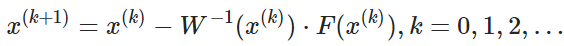
\includegraphics[scale = 0.70]{images/p3_6_1.png}
	\label{image:p3_6_1}
\end{figure}

\subsection{Решение задачи через нормирующую константу методом Ньютона}

Решение задачи через нормирующую константу методом Ньютона c начальным приближением (Приложение 11).

Результат решения задачи методом Ньютона c начальным приближением $u=[10, 10, 10, 10]$ и значением ошибки $e=1e^{-6}$:

\lstinputlisting{listings/p3.l3.log}

Алгоритм успешно сходится за 16 итераций. С каждой итерацией алгоритма значения целевых функций стемятся к нулю, результирующая цена также постепенно уменьшается.

\section{Вывод}

Как и ожидалось, алгоритм простых итераций не сходится, поэтому пришлось использовать более надежный алгоритм Ньютона. Модифицированный алгоритм Ньютона чрезвычайно чувствителен к выбору начального приближения, поэтому был использован вариант алгоритма с расчетом матрицы Якоби. Для увеличения производительности данного алгоритма можно подключить пакет MATLAB Parallel Computing Toolbox, который использует MPI для эффективного распараллеливания. 